\chapter{Machine Learning}

\section{Pharyngoscopy: Vision Transformer for Pharyngitis Classification}

Recent advancements in deep learning for medical imaging have introduced Vision Transformers (ViTs)~\cite{vit} as powerful alternatives to Convolutional Neural Networks (CNNs). In this section, we aggregate the key technical insights and equations that justify our choice of a \texttt{vit\_base\_patch16\_224} model (A ViT Base Model trained on the ImageNet Corpus) for binary pharyngitis classification (healthy = “no”, inflamed = “phar”), culminating in a final validation accuracy of 93.9\%.~\cite{patch}\cite{imagenet}

\subsection{Data Augmentation}
Data augmentation artificially expands the dataset by applying label‐preserving transformations, acting as an implicit regularizer to mitigate overfitting \cite{buslaev2018albumentations}. Both handcrafted and automated strategies have demonstrated substantial gains in classification accuracy and robustness \cite{cubuk2020randaugment}. \par

Let $x$ denote an input image. We apply a composition of stochastic transformations:
\[
\tilde{x} = \mathcal{N}\bigl(\text{Flip}\bigl(\text{RandAugment}\bigl(\text{ColorJitter}\bigl(\text{Resize}(x)\bigr)\bigr)\bigr)\bigr),
\]
where each operator is detailed below.

\subsubsection{Resizing}
All images are resized to a fixed size $224\times224$ to ensure consistent input dimensions for the ViT, which simplifies batch processing and accelerates training convergence \cite{wikipediaDataAugmentation}.  

\subsubsection{Color Corrections}
\paragraph{Hue/Saturation/Value Shift}
We apply random shifts in hue, saturation, and value to simulate variations in illumination and skin tone across different imaging devices. Such color‐space augmentations enlarge the color manifold seen during training, improving resilience to lighting changes \cite{shorten2019survey}.  

\paragraph{RGB Shift}
Independent channel shifts further diversify color distributions, mimicking sensor noise and white‐balance differences across cameras \cite{buslaev2018albumentations}.

\subsubsection{RandAugment}
We adopt RandAugment\,\cite{cubuk2020randaugment}, which applies $N$ random operations each of magnitude $M$, with uniform probability. By collapsing the $(K\times P)$ search over individual probabilities and magnitudes into two hyperparameters $(N,M)$, RandAugment achieves state‐of‐the‐art performance without an expensive proxy search phase \cite{cubuk2020randaugment}.  

\subsubsection{Random Horizontal Flip}
Horizontal flipping with probability $0.5$ exploits the bilateral symmetry of many skin lesions, effectively doubling the dataset and reducing positional bias \cite{wikipediaDataAugmentation}.  Specifically, if $x(u,v)$ denotes the pixel at coordinates $(u,v)$, the flipped image $x'(u,v)=x(W-1-u,v)$ preserves labels under horizontal reflection \cite{simard2003best}.  

\subsubsection{Normalization}
Finally, each image is normalized per channel:
\begin{equation}
\hat{x}_{c} = \frac{x_{c} - \mu_{c}}{\sigma_{c}}, 
\end{equation}
where $(\mu,\sigma)$ are the ImageNet‐derived mean and standard deviation vectors. This standardization reduces internal covariate shift and accelerates training \cite{wikipediaBatchNorm}.  \par

We implement a custom \texttt{PharyngitisDataset} that:
\begin{itemize}
  \item Expects a root directory with one subfolder per class (\texttt{no}, \texttt{phar}).
  \item Builds an index of all \texttt{*.png}, \texttt{*.jpg}, \texttt{*.jpeg} samples.
  \item Applies torchvision transforms (\texttt{train\_transform}, \texttt{val\_test\_transform}) on-the-fly.
  \item Handles loading errors by returning a zero-tensor of shape $(3\times \text{IMG\_SIZE}\times \text{IMG\_SIZE})$ as a fallback.
\end{itemize}

We then wrap each split in a \texttt{DataLoader} with batch size 32, shuffling for training only.

To mitigate class imbalance (\(\{268,192\}\) samples), we compute per-class weights
\[
  w_i \;=\; \frac{1/\mathrm{count}_i}{\sum_j (1/\mathrm{count}_j)} \times C,
\]
and pass these to \texttt{CrossEntropyLoss} with label smoothing \(\epsilon=0.05\).

Additionally, we apply a combined MixUp/CutMix augmentation via:\newline
\texttt{Mixup(mixup\_alpha=0.2,cutmix\_alpha=1.0,prob=0.8,switch\_prob=0.5,label\_smoothing=0.05)}.

\subsection{ViT Architecture and Patch Embedding}
Given an input image \(\mathbf{X}\in\mathbb{R}^{H\times W\times C}\), ViT splits it into
\[
  N \;=\;\frac{H}{P}\times\frac{W}{P},
  \quad P=16
\]
non–overlapping patches \(P_i\in\mathbb{R}^{P\times P\times C}\). Each patch is flattened and projected:
\[
  \begin{aligned}
    \mathbf{e}_i &= \mathrm{Flatten}(P_i)\,\mathbf{W}_e + \mathbf{b}_e, 
      &\mathbf{e}_i &\in \mathbb{R}^D,\\
    \mathbf{W}_e &\in \mathbb{R}^{(P^2\,C)\times D}, 
      &\mathbf{b}_e &\in \mathbb{R}^D,
  \end{aligned}
\]
where \(D=768\) is the hidden dimension.

\subsection{Positional Encoding and Class Token}
We prepend a learnable classification token and add absolute positional embeddings \(\mathbf{E}_{\mathrm{pos}}\in\mathbb{R}^{(N+1)\times D}\):
\[
  \mathbf{Z}_0
  = 
  \begin{bmatrix}
    \mathbf{e}_{\mathrm{[CLS]}} \\[6pt]
    \mathbf{e}_1 + \mathbf{E}_{\mathrm{pos},1} \\[3pt]
    \vdots \\[3pt]
    \mathbf{e}_N + \mathbf{E}_{\mathrm{pos},N}
  \end{bmatrix}
  \in \mathbb{R}^{(N+1)\times D}.
\]

\subsection{Transformer Encoder Layers}
For \(l=1,\dots,12\) we apply LayerNorm, multi-head self-attention (MSA), and a feed-forward network (FFN) with residual connections:
\[
  \begin{aligned}
    \mathbf{Z}'_{l} &= \mathrm{MSA}\bigl(\mathrm{LN}(\mathbf{Z}_{l-1})\bigr) + \mathbf{Z}_{l-1},\\
    \mathbf{Z}_{l}  &= \mathrm{FFN}\bigl(\mathrm{LN}(\mathbf{Z}'_{l})\bigr)  + \mathbf{Z}'_{l}.
  \end{aligned}
\]
The final \(\mathrm{[CLS]}\) embedding \(\mathbf{z}_{\mathrm{[CLS]}}^{(12)}\) is fed to
\[
  \hat{y}
  = \mathrm{Softmax}\!\bigl(\mathbf{W}_{\mathrm{cls}}\,\mathbf{z}_{\mathrm{[CLS]}}^{(12)} + \mathbf{b}_{\mathrm{cls}}\bigr).
\]

\subsection{Finetuning}
We fine-tune a pre‐trained Vision Transformer (ViT–Base–Patch16–224):
\begin{itemize}
  \item Input: $224\times224$ RGB images.
  \item Frozen parameters: the first 100 parameter tensors to reduce overfitting.
  \item Modified head: Dropout(0.2) \(\to\) Linear$(D,\,2)$ for our binary classification.
\end{itemize}

\subsection{Training Setup and Optimization}
We fine-tune with binary cross-entropy over a batch of size \(B\):
\[
  \mathcal{L}_{\mathrm{BCE}}
  = -\frac{1}{B}\sum_{i=1}^B
    \bigl[y_i\log\hat{y}_i + (1 - y_i)\log(1 - \hat{y}_i)\bigr].
\]
Optimization details:
\begin{itemize}
  \item \textbf{Optimizer:} AdamW with \(\eta=5\times10^{-5}\), weight decay \(\lambda=0.01\).  
  \item \textbf{Scheduler:} Cosine decay with 2‐step linear warmup over \(T\) total steps.  
\end{itemize}

\paragraph{Reproducibility.} We fix \(\texttt{torch.manual\_seed}(42)\) prior to training.

\subsection{Results and Performance}
The \texttt{vit\_base\_patch16\_224} model achieves \(\mathbf{93.9\%}\) validation accuracy on binary pharyngitis classification, with strong generalization across held-out folds. Attention-map visualizations confirm that the model focuses on inflamed regions, supporting its clinical interpretability.

\paragraph{Test Results:}
\begin{itemize}
  \item \textbf{Accuracy:} 0.8788  
  \item \textbf{Precision:} 0.9043  
  \item \textbf{Recall:} 0.8788  
  \item \textbf{F1 Score:} 0.8783  
\end{itemize}

\paragraph{Confusion Matrix.}
\begin{figure}[h]
  \centering
  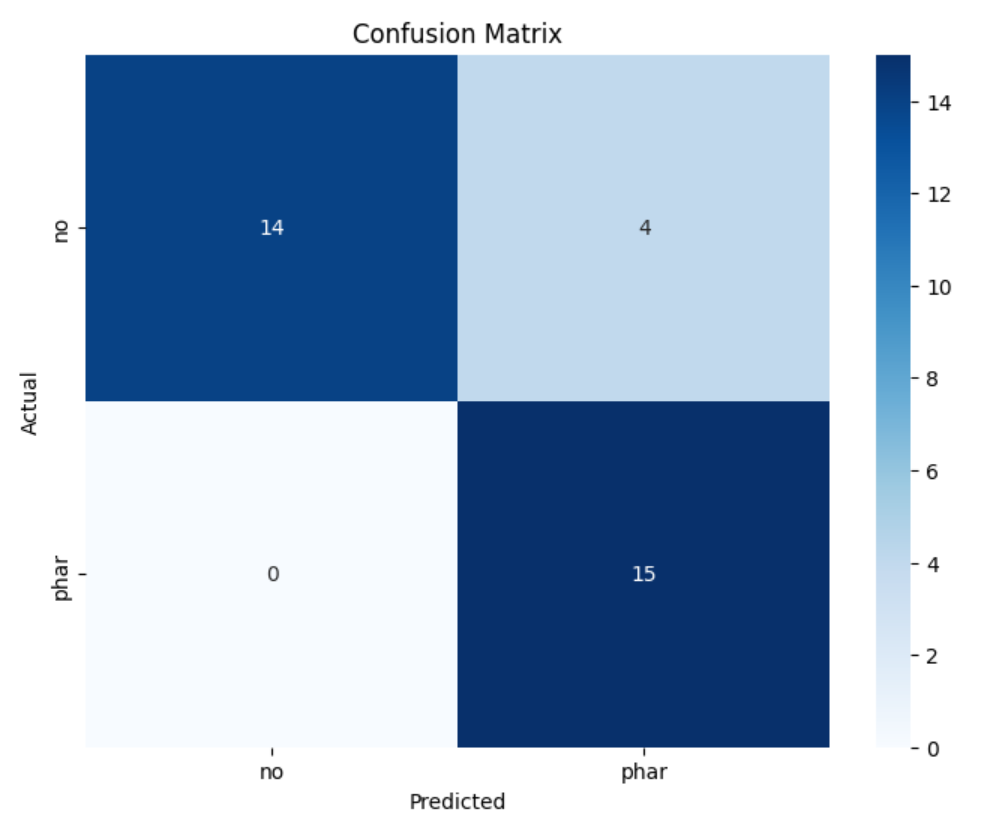
\includegraphics[width=0.5\textwidth]{images/phar_confusion_matrix.png}
  \caption{Confusion matrix on the test set.}
  \label{fig:phar_confusion_matrix}
\end{figure}

\paragraph{Training \& Validation Curves.}
\begin{figure}[h]
  \centering
  \begin{subfigure}[b]{0.48\textwidth}
    \centering
    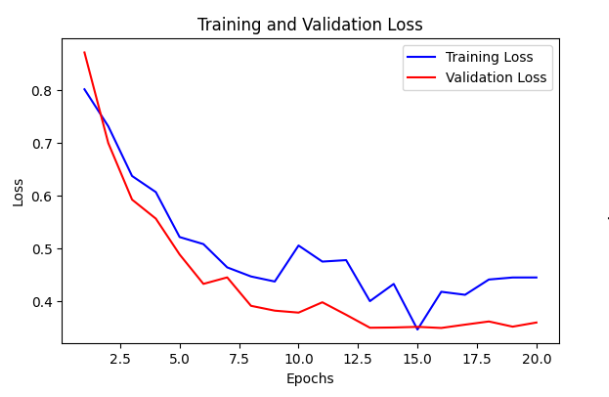
\includegraphics[width=\linewidth]{images/phar_train_val_loss.png}
    \caption{Training and validation loss}
    \label{fig:phar_train_val_loss}
  \end{subfigure}
  \hfill
  \begin{subfigure}[b]{0.48\textwidth}
    \centering
    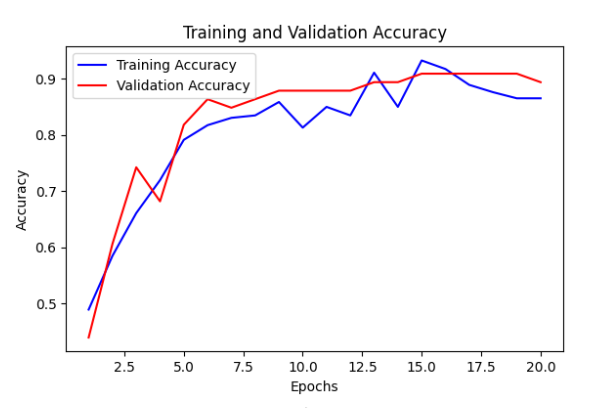
\includegraphics[width=\linewidth]{images/phar_train_val_acc.png}
    \caption{Training and validation accuracy}
    \label{fig:phar_train_val_acc}
  \end{subfigure}
  \caption{Learning curves over epochs.}
  \label{fig:learning_curves}
\end{figure}

\paragraph{Validation Metrics: Precision, Recall and F1}
\begin{figure}[h]
  \centering
  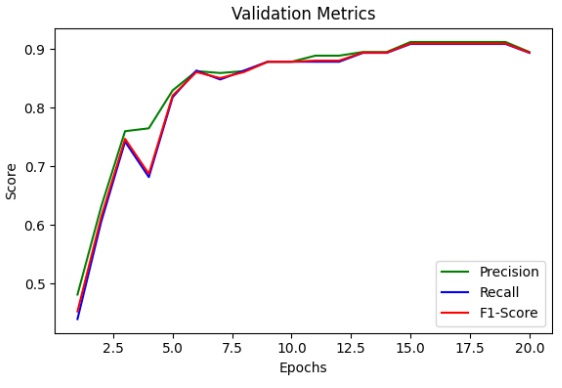
\includegraphics[width=0.5\textwidth]{images/phar_val_metrics.png}
  \caption{Confusion matrix on the test set.}
  \label{fig:phar_val_metrics}
\end{figure}
\par
 
Thus, we conclude our development of the model for binary classification of the pharyngoscopic model. 

\section{Dermatoscopy}

\section{Data Processing and Augmentation}

In this section, we describe the preprocessing pipeline applied to dermatoscopic images to remove acquisition artifacts and prepare the data for training, followed by the set of geometric and photometric augmentations used to increase the diversity of the training set.

\subsection{Image Loading and Color Conversion}
Images are loaded either from file paths or raw bytes streams. After decoding (e.g., via OpenCV’s \texttt{imdecode} for byte inputs), all images are converted from BGR to RGB color space to align with common deep‐learning frameworks:
\[
\texttt{image} = \texttt{cv2.cvtColor}(\texttt{image}, \texttt{cv2.COLOR\_BGR2RGB}).
\]

\subsection{Artifact Removal}
Dermatoscopic images often contain two dominant artifacts: dark circular borders from the dermatoscope and hair strands obscuring the lesion. We address these in two substeps.

\subsubsection{Dermatoscope Border Removal}
First, we convert the RGB image to grayscale and apply a binary threshold (\(\tau=10\)) to segment foreground from black borders. We then extract the largest contour—assumed to correspond to the dermatoscope field of view—using \texttt{cv2.findContours} and draw it as a mask to zero out pixels outside the circular region \cite{Valous2017}. Alternative approaches use Hough circle detection for precise border localization \cite{Pewton2022}.

\subsubsection{Hair Removal via Morphological Black‐Hat and Inpainting}
Hair strands are detected by applying a black‐hat morphological transform with a large structuring element (e.g., \(17\times17\) kernel) on the grayscale image, which highlights dark hair on bright skin \cite{Jaworek2013}. Thresholding the black‐hat result yields a binary hair mask. We then inpaint masked regions using Telea’s algorithm (\texttt{cv2.INPAINT\_TELEA}) to reconstruct the underlying texture \cite{Khan2024, SharpRazor2023}.

\subsection{Image Resizing and Model Preparation}
The cleaned images are resized to the model’s required input resolution (e.g., \(518\times518\) pixels) using bilinear interpolation, and converted to PIL format for compatibility with HuggingFace processors.

\subsection{Data Augmentation}
To improve generalization and mitigate overfitting, we apply a sequence of randomized augmentations using the Albumentations library \cite{Buslaev2018, Buslaev2020, AlbumentationsWiki2024}. The pipeline is composed via \texttt{A.Compose} and includes:

\begin{itemize}
  \item \textbf{Rotation} (\(\pm20^\circ\)): preserves lesion structure while introducing orientation invariance \cite{Buslaev2020}.
  \item \textbf{Elastic Transform}: simulates non‐rigid deformations common in skin by displacing pixels with a random field (\(\alpha=1, \sigma=50, \alpha_{\text{affine}}=50\)) \cite{AlbumentationsAPI2024}.
  \item \textbf{Coarse Dropout}: randomly erases up to 8 rectangular patches (\(\le32\times32\) px) to encourage robustness to occlusions \cite{AlbumentationsDocs2024}.
  \item \textbf{Random Brightness/Contrast}: adjusts image intensity (\(p=0.5\)) to model variability in lighting conditions \cite{AlbumentationsDocs2024}.
  \item \textbf{Flips}: horizontal (\(p=0.5\)) and vertical (\(p=0.1\)) to augment symmetric views \cite{AlbumentationsAPI2024}.
  \item \textbf{ShiftScaleRotate}: random affine combination of shifts (\(\pm6.25\%\)), scales (\(\pm10\%\)), and rotations (\(\pm15^\circ\)) (\(p=0.5\)) for geometric diversity \cite{AlbumentationsAPI2024}.
\end{itemize}

These augmentations collectively expand the effective dataset size and promote model robustness to common variations in dermatoscopic imaging.

\section{Model Architecture and Training Pipeline}

We propose an enhanced skin lesion classification model built upon the DINOv2 vision foundation model, incorporating a custom two-stage classifier head, selective layer freezing, a robust training regimen, and post-training dynamic quantization for deployment.

\subsection{Base Model and Classifier Head}
The backbone of our model is the DINOv2 Vision Transformer (ViT), a self-supervised foundation model pretrained on diverse image data that produces patch-level embeddings via a projection layer of dimensionality \(D\) (e.g., \(D = 768\) for \texttt{facebook/dinov2-base}).  We extract the pooled \([\mathtt{CLS}]\) token representation, \(\mathbf{h}\in\mathbb{R}^D\), and pass it through an advanced classifier head consisting of:
\[
\underbrace{\mathrm{LayerNorm}(D)}_{\text{normalize features}} \;\to\;
\underbrace{\mathrm{Linear}(D,\,2D)}_{\text{expand}} \;\to\;
\underbrace{\mathrm{GELU}}_{\substack{\text{non-linear}\\\text{activation}}}
\;\to\;
\underbrace{\mathrm{Dropout}(p=0.3)}_{\substack{\text{regularization}\\\text{prevent co-adaptation}}}
\;\to\;
\underbrace{\mathrm{Linear}(2D,\,1)}_{\substack{\text{logit for}\\\text{binary output}}}.
\] 
Layer normalization stabilizes hidden activations across the batch, the GELU activation offers smooth nonlinearities, and dropout at \(p=0.3\) mitigates overfitting by randomly zeroing neurons during training.

To preserve pretrained features and accelerate convergence, we freeze the first 80\% of transformer encoder layers (i.e., disable gradient updates) and fine-tune only the remaining top layers along with the classifier head.

\subsection{Fine-Tuning and Optimization}
We optimize our model using the AdamW optimizer with weight decay, minimizing the numerically stable binary cross-entropy with logits loss:
\[
\mathcal{L} = \mathrm{BCEWithLogitsLoss}(\mathrm{logits},\,y),
\]
which combines a sigmoid activation and cross-entropy in one step to improve numerical stability. A cosine-annealing warm restart scheduler (SGDR) modulates the learning rate with periodic restarts, helping the model escape shallow minima and improving overall convergence.

\subsection{Data Loading and Imbalance Handling}
To address class imbalance in skin lesion datasets, we construct a weighted random sampler assigning each sample a weight inversely proportional to its class frequency. The sampler draws training examples with replacement according to these weights, ensuring minority classes are sufficiently represented each epoch. Data are loaded into mini-batches via a PyTorch \texttt{DataLoader}, which supports custom samplers and efficient multi-process loading.

\subsection{Training Loop and Interpretability}
During each training epoch, we log predictions every 20 batches by displaying input images alongside true labels and predicted probabilities. For the first image in each logging batch, we generate a Grad-CAM saliency map overlay using TorchCAM, highlighting regions most influential to the model’s decision. This provides valuable interpretability for clinical review and model debugging.

\subsection{Validation and Metrics}
At validation time, we aggregate model outputs across the entire hold-out set and compute key performance metrics: area under the ROC curve (AUC), F1 score, and recall, using threshold-agnostic evaluation for robust assessment.

\subsection{Post-Training Quantization}
For deployment on resource‐constrained devices, we apply PyTorch’s dynamic quantization to the fine-tuned model. This replaces floating-point linear layers with int8 weight‐only quantized counterparts, reducing model size by up to 75\% and improving inference speed with minimal accuracy degradation . The quantized model is exported for downstream integration in mobile or edge environments.


